\documentclass[final]{siamltex}

\usepackage{amssymb}
\usepackage{amsmath}
\usepackage{mathtools}
\usepackage{latexsym}
\usepackage{graphicx} % Changed the graphics package but can be changed back if needed?
\graphicspath{{Images/}}
\usepackage{url}
\usepackage{xcolor}
\usepackage[boxed]{algorithm}
\usepackage{algpseudocode}
\usepackage[warning,debug,nosepfour,autolanguage]{numprint}

\newtheorem{Def}{Definition}
\newtheorem{Thm}{Theorem}
\newtheorem{Lem}{Lemma}
\newtheorem{Rem}{Remark}

\newcommand{\adja}{q_a}
\newcommand{\adjb}{q_b}
\newcommand{\adjaB}{q_{a,\partial \Omega}}
\newcommand{\adjbB}{q_{b,\partial \Omega}}
\newcommand{\adjB}{q_{\partial \Omega}}
\newcommand{\Adja}{\mathbf{p}}
\newcommand{\Adjb}{q}
\newcommand{\adj}{q}
\newcommand{\Adjc}{{q}_{\partial \Omega}}
\newcommand{\ra}{\rho_a}
\newcommand{\rb}{\rho_b}
\newcommand{\w}{\vec{w}}
\newcommand{\f}{\mathbf{f}}
\newcommand{\ve}{\mathbf{v}}
\newcommand{\n}{\vec{n}}
\newcommand{\h}{\mathbf{h}}
\newcommand{\K}{\mathbf{K}}
\newcommand{\x}{\vec{x}}
\newcommand{\F}{\mathcal{F}}
\newcommand{\hr}{\widehat \rho}


\title{PDE-Constrained Optimization for Dynamical Density Functional Theory Modelling Sedimentation Processes}

	\author{Benjamin D. Goddard\thanks{The School of Mathematics and Maxwell Institute for Mathematical Sciences, The University of Edinburgh, Edinburgh, EH9 3FD, UK ({\tt b.goddard@ed.ac.uk})} 
	%
	\and John W. Pearson\thanks{The School of Mathematics and Maxwell Institute for Mathematical Sciences, The University of Edinburgh, Edinburgh, EH9 3FD, UK ({\tt j.pearson@ed.ac.uk})} 
	%
	\and Jonna C. Roden\thanks{The School of Mathematics and Maxwell Institute for Mathematical Sciences, The University of Edinburgh, Edinburgh, EH9 3FD, UK ({\tt J.C.Roden@sms.ed.ac.uk})}}

\begin{document}
	\maketitle
	
	\begin{abstract}
		Abstract
	\end{abstract}
	
	\begin{keywords}PDE-constrained optimization; Multiscale particle dynamics; Pseudospectral methods\end{keywords}
	
	\begin{AMS}--\end{AMS}
	
	
	\pagestyle{myheadings}
	\thispagestyle{plain}
	\markboth{B. D. GODDARD, J. W. PEARSON, AND J. C. RODEN}{PDE-CONSTRAINED OPTIMIZATION FOR DDFT}
	
	
\section{Introduction}\label{sec:Intro}
The aim of this work is to solve optimal control problems involving particle dynamics models, which describe sedimentation processes. This is of interest in various contexts of biology and industry, such as in brewing and +++. This paper is based on +++ cite our paper +++, which introduced a fast and efficient numerical scheme, based on pseudospectral methods and a sweeping algorithm, to solve optimal control problems involving multiscale particle dynamics models. In the previous work, only advection-diffusion equations with mean-field type particle interactions were investigated. In this paper, this method is extended to tackle more complex models which can describe sedimentation processes.

Dynamical Density Functional Theory (DDFT) is a successful framework for modelling colloidal fluids by considering the free energy functional of a system, which only depends on a one-body particle distribution $\rho$. This theory can be used in a wide range of applications, such as ++,++,++, and also to model sedimentation processes. Most work on sedimentation, see ++,++, employs Rosenfeld's Fundamental Measure Theory (FMT) \cite{RosenfeldFMT}, which is a Density Functional Theory (DFT) for hard sphere mixtures.
Based on this theory for three dimensional spheres and the fact that the theory for hard rods is known exactly \cite{Percus1976}, Rosenfeld \cite{Rosenfeld2DInterp} derived an approximation of this theory for two dimensional hard disks and showed that in the uniform limit, for one particle species, we get the approximate free energy density
\begin{align} \label{eqn:SPTFunctional2D}
	\Phi = - \rho \ln (1- \eta) + \frac{\rho \eta}{1 - \eta} = \rho \left(-\ln(1-\eta) + \frac{1}{1- \eta} -1 \right),
\end{align} 
where $\eta = a \rho = \frac{\pi \sigma^2}{4} \rho$, and $\sigma$ the particle diameter of the hard sphere particle.
This expression for the free energy for the bulk fluid is the same as derived by scaled particle theory (SPT) \cite{Reiss1959}, \cite{Reiss1960}, \cite{Helfand1961}, which also coincides with the Percus-Yevic compressibility equation \cite{PercusYevick1}, as detailed in \cite{RosenfeldSPT}.
While the SPT approximation \eqref{eqn:SPTFunctional2D} and its three-dimensional equivalent are used in classical DFT, see \cite{DFTWinkelmann2001}, \cite{DFTRoth1}, \cite{DFTRoth2}, \cite{DFTGonzalez1997}, \cite{DFTCuesta2008}, \cite{DFTLoewen2002}, and other statistical mechanics approaches, see for example \cite{GrafLoewen1999}, \cite{DuBois2002}, \cite{Chamoux1998}, \cite{Chamoux1996}, in dynamical DFT it is not commonly applied and only the work of Archer et al. \cite{ArcherSed1}, \cite{ArcherSed2008}, \cite{ArcherSed2011}, \cite{ArcherSed2013}, is known to us in this context. Archer and Malijevs\'y \cite{ArcherSed1} used this SPT approximation in their DDFT model to describe sedimentation processes. This reduces computational cost significantly, in comparison with computing the full FMT version, by avoiding the computation of convolution integrals for the fundamental measures, while still obtaining very good results compared to Brownian dynamics simulations. 
In this paper, we apply this type of sedimentation model as the constraint for an optimal control problem. While there are many applications of PDE-constrained optimization, such as ++, ++, ++, to our knowledge, there does not exist work on optimization involving DDFT models. We want to minimize a cost functional, which measures the closeness between the particle distribution, or state, and a desired state, as well as a control term, which enters the model equation as a background flow. We will consider a time-dependent and a time-independent control, i.e. a problem set-up where the flow is allowed to vary over time, and one where it is held constant over the whole time horizon $(0,T)$.  

This paper is organised as follows. In Section \ref{sec:FWModel} we introduce the relevant model equations based of those used in \cite{ArcherSed1}. In Section \ref{sec:OCP} the optimal control problem we want to solve is formulated and first order optimality conditions are derived. Following this, the numerical methods used to solve this optimality system are discussed in Section \ref{sec:Methods} followed by numerical experiments in Section \ref{sec:Expts} before closing with some remarks in Section \ref{sec:Conc}.

\section{Model Equations}\label{sec:FWModel}
We are interested in modelling sedimentation processes using DDFT following the work by Archer and Malijevs\'y \cite{ArcherSed1}. 
In order to extend this work to optimal control problems, in this paper an additional advection term is added to the model in \cite{ArcherSed1}. The considered model describes the dynamics of a particle density $\rho(\x, t)$, given an initial condition $\rho(\x,0)$, on some domain $\Omega$ and time interval $(0,T)$. This is
\begin{align}\label{Eq1}
	&\partial_t \rho = \sigma^2\nabla \cdot \left(  \rho \nabla \frac{\delta \F[\rho]}{\delta \rho} - \rho \w  \right): = - \sigma^2\nabla \cdot \vec j \quad \text{in} \quad \Omega \times (0,T).
\end{align}
 The free energy functional is identical to the one considered in \cite{ArcherSed1}
\begin{align*}
	\F[\rho] &= \int  \rho (\ln \Lambda^2 \rho - 1)  + \Phi + \rho V_{ext}  d \x + \frac{1}{2}\int \int \rho(\x) \rho(\x') V_2(|r - r'|) d\x d\x',
\end{align*}
where the approximate free energy density \eqref{eqn:SPTFunctional2D} describes the volume exclusion through hard disks. The external potential is defined as $V_{ext} = c y$, where $c$ is the constant strength of the potential force acting on the particles. Furthermore, we have the pair potential $V_2 = \kappa \exp(-|\x|/\sigma)$, where $\kappa$ is a constant determining the particle interaction strength. Expressing the functional derivative explicitly, we get the following model describing particle dynamics influenced by mean-field interactions, volume exclusion, external forces, advection and diffusion
\begin{align} \label{eq:SedFWModel}
	\partial_t \rho =&  \mathcal{D}(\rho,\w),
\end{align}
where
\begin{align*} 
	\mathcal{D}(\rho,\w):=&\sigma^2  \bigg( \frac{\nabla^2 \rho}{1 - \eta} +  \nabla \rho \cdot \nabla \frac{(3- 2 \eta)}{(1 - \eta)^2}  - \rho \nabla^2\frac{\eta - 2}{(\eta - 1)^2}  \\
	&-  \nabla \cdot \left( \rho \w  \right) +  \nabla \cdot \left( \rho \nabla V_{ext}\right) + \int \rho(\x) \rho(\x') \nabla V_2(|\x - \x'|)d\x'\bigg). \notag
\end{align*}
Different boundary conditions can be applied to this model, and in ++ our paper ++ the formalism for Dirichlet and no-flux boundary conditions was introduced. In this work, we restrict our attention to no-flux boundary conditions, since they are more relevant to physical applications. +++++ periodic ??? ++++
The no flux boundary conditions for this problem read
\begin{align}\label{eq:noFluxBCs}
	- \vec j \cdot \n = 0 \quad \text{on} \quad \partial \Omega,
\end{align}
where $\vec j$ is defined in \eqref{Eq1} and $\n$ is the outward normal.
\section{The PDE-Constrained Optimization Problem and the Resulting Optimality System}\label{sec:OCP} 
In PDE-constrained optimization, we are interested in minimizing a cost functional $\mathcal J$, which measures the distance between the particle density $\rho$ and a desired particle state $\hr$ as well as the size of a control $\w$. The two terms are measured in an $L_2$ norm in space and an $L_1$ norm in time. The minimization of the cost functional is subject to a constraint, which is given by the PDE model that we are considering. In this work, the control enters the PDE model in the advection term. A regularization parameter $\beta$ penalizes the use of the control, so that for large values of $\beta$, little control can be introduced into the system and vice versa. 
We consider the cost functional
\begin{align}\label{eq:OCP1}
	& \min_{\rho,\w}\mathcal J(\rho, \w) := \frac{1}{2}\int_0^T \int_\Omega (\rho - \widehat \rho)^2 d\x dt + \frac{\beta}{2} \int_0^T\int_\Omega \w^2 d\x dt,
\end{align}
which is minimized subject to the constraint \eqref{eq:SedFWModel} with boundary conditions \eqref{eq:noFluxBCs}.
We can then define the Lagrangian of this problem as follows
\begin{align*}
	\mathcal{L} (\rho,\w,\adj_1, \adj_2) = \mathcal J(\rho, \w) - \int_0^T \int_\Omega \left( \partial_t \rho - \mathcal{D}(\rho,\w) \right) \adj_1 d\x dt - \int_0^T \int_{\partial \Omega} \vec j \cdot \n \adj_2  d\x dt.
\end{align*}
Following the standard method for deriving an optimality system for parabolic PDEs, for example described in ++ ++, the stationary states of the system have to be found by computing the derivatives of the Lagrangian with respect to each of the variables. Computing this with respect to the adjoint variables $\adj_1$ and $\adj_2$, the forward model \eqref{eq:SedFWModel} and boundary conditions \eqref{eq:noFluxBCs} are retrieved. Evaluating $D_\rho \mathcal{L} (\rho,\w,\adj_1, \adj_2)\rho = 0$, the derivative with respect to $\rho$, results in the adjoint equation. A relationship between $\adj_1$ and $\adj_2$ is found in the process, so that in the following the indices are dropped for notational convenience.
The adjoint equation reads
\begin{align}\label{eq:SedAdjointEq}
	\frac{\partial q}{\partial t} = \mathcal{D}^*(\adj,\w),
\end{align}
where
\begin{align*}
	\mathcal{D}^*(\adj,\w): =& \sigma^2 \bigg(\frac{(-1 + 5 a \rho - 2 a^2 \rho^2) }{(a \rho -1)^3}\nabla^2 q + \frac{4 a \nabla \rho }{(a \rho -1)^3}\cdot \nabla q + \frac{2 a   \nabla^2 \rho}{(a \rho -1)^2} q - \w \cdot \nabla q \\
	&+ \nabla V_{ext} \cdot \nabla q 
	- \rho + \hr + \int \left(\nabla_r q(r) - \nabla_{r'} q(r') \right) \rho(r') \nabla V_2(|\x -\x'|) d\x' \bigg),
\end{align*}
with $q(\x,T) =0$, a final time condition at $t =T$.
We further have the boundary condition
\begin{align*}
	\frac{(1 + a \rho) \nabla q}{(a \rho -1)^3}\cdot \n = 0.
\end{align*}
Since $a \rho >0$ by definition, this is
\begin{align}\label{eq:noFluxAdjBCs}
	\frac{\partial q}{\partial n} = 0.
\end{align}
By solving the third condition $D_{\w} \mathcal{L} (\rho,\w,\adj_1, \adj_2)\w = \vec 0$ the so called gradient equation is derived. This results in
\begin{align}\label{eq:SedGradientEq}
	\w = - \frac{1}{\beta}\rho \nabla q.
\end{align}
The first-order optimality system that needs to be solved simultaneously consists of the forward model \eqref{eq:SedFWModel} with boundary conditions \eqref{eq:noFluxBCs}, the adjoint equation \eqref{eq:SedAdjointEq} with boundary conditions \eqref{eq:noFluxAdjBCs} and the gradient equation \eqref{eq:SedGradientEq}.

We can modify the cost functional to include a time independent control, which only depends on the position $\x$. This reads
\begin{align}\label{eq:OCP2}
	& \min_{\rho,\w}\mathcal J(\rho, \w) := \frac{1}{2}\int_0^T \int_\Omega (\rho - \widehat \rho)^2 d\x dt + \frac{\beta}{2} \int_\Omega \w(\x)^2 d\x,
\end{align}
again, subject to the constraint \eqref{eq:SedFWModel} with boundary conditions \eqref{eq:noFluxBCs}.
When deriving the optimality system for the problem involving the cost functional \eqref{eq:OCP2}, the adjoint equation remains the same, however, the gradient equation changes to be
\begin{align} \label{eq:SedGradientEq2}
	\w(\x) = - \frac{1}{\beta} \int_0^T \rho  \nabla q dt.
\end{align}
When comparing this with the time-dependent gradient equation \eqref{eq:SedGradientEq}, we can observe that the time-independent control is enforced by averaging the gradient equation with respect to time. ++ time independent control ref? +++
\section{Numerical Methods}\label{sec:Methods}
In the following, each aspect of the numerical method for solving the optimal control problem is introduced briefly. For a more thorough discussion we refer to ++our paper++. 
The space and time discretization of the domain, the creation of integration and interpolation vectors, as well as convolution and differentiation matrices involved in solving the optimality system are done using pseudospectral methods. This is implemented using the code library 2DChebClass, see \cite{GoddardPseudospectralCode1} for a detailed account of the method. Pseudospectral methods are collocation methods, which, in this case, employ interpolation using Lagrange polynomials on a Chebyshev grid. This results in exponential accuracy for smooth functions and is efficient in solving non-linear, non-local PDEs, since they produce small dense matrices. This is an advantage over using Finite Element Methods, since these would involve dealing with large matrices, which would not be sparse due to the non-local integral term, losing the key advantage of applying this method. Furthermore, Clenshaw-Curtis weights are used for creating integration vectors. 
Boundary conditions of the PDE are imposed by extending the discretized PDE by an algebraic equation, so that we are solving an algebraic-differential equation. This is done in {Matlab}, using the algebraic-differential ODE solver \texttt{ode15s}. 

One subtlety to be noticed here is that in the derivation of the adjoint PDE, a final time condition is found, as opposed to an initial condition. This also causes issues with the numerical stability of the problem, due to a negative Laplacian term. We circumvent these issues by a change of time variable. This results in the adjoint PDE running backward in time, with an initial condition at $t = T$, compared to the forward model, which has an initial condition at $t = 0$. 
In order to solve the optimality system, consisting of the forward and adjoint PDEs as well as the gradient equation, we apply a sweeping algorithm.
This algorithm is initialized by an initial guess for the control $\w^0$. Using this, the forward model is solved using pseudospectral methods. Then, using the resulting state $\rho$, we can solve the adjoint equation. The gradient equation provides a way of updating the control $\w$, provided with the state $\rho$ and the adjoint variable $\adj$ from solving the two PDEs. This update $\w^{i}_g$ is not immediately given to the algorithm as a new initial guess, but is mixed with the previous iterate of $\w$ to provide more numerical stability. The update $\w^{i+1}$ is calculated by taking the linear combination of the previous iterate $\w^{i}$ and the result from the gradient equation $\w^{i}_g$ by calculating
\begin{align*}
	\w^{i+1} = (1 - \lambda) \w^{i} + \lambda \w^{i}_g,
\end{align*}
where $\lambda$ is a mixing parameter in $[0,1]$, which is set to be $0.01$ for most problems.
The algorithm converges if the error between $\w^{i}$ and $\w^{i+1}$ is smaller than some chosen tolerance. All errors are measured using an $L_2$ norm in space and an $L_\infty$ norm in time. The relative error has a factor of $10^{-10}$ added in the denominator to avoid dividing by zero. The final error measure considers the minimum of the absolute and the relative error between the two iterates, in order to account for erroneously inflated relative errors caused by dividing by small quantities.
+++ multishape?+++
\section{Numerical Experiments}\label{sec:Expts}
+++ do we include validation against archer anywhere? +++
In the following we solve several examples of optimal control problems that are constrained by the proposed DDFT model. Each of these examples will model particles under the influence of a gravitational force and with attractive particle interactions, which are sedimenting and clustering over the time horizon. First we consider examples in a box-shaped domain. Then we demonstrate the functionality of the code on a multishape domain. The extension of the method to multishape domains is explained in ++?++.
\subsection{Optimization in a Box}
We consider the time-dependent optimal control problem \eqref{eq:OCP1} subject to the constraint \eqref{eq:SedFWModel} with boundary conditions \eqref{eq:noFluxBCs}.
At first we set up a test problem which sets $\hr$ to be the forward solution for a problem with $V_{ext} = cy$, where $c = 0.1$, where the interaction strength $\kappa = -3.5$ and the initial condition for $\rho$ is $\bar \rho = 0.036$, with a particle diameter $\sigma = 1$. These values are chosen to align with those in \cite{ArcherSed1}.
We have $N = 40$ discretization points in space and $n = 30$ points in time. The chosen domain is $[0,30] \times[0,20]$ and the time horizon is $(0,300)$. We choose an ODE tolerance of $10^{-7}$, the optimization tolerance is $10^{-3}$ and the mixing parameter is $\lambda = 0.01$. 
We initialize the optimization routine with the initial guess for $\w$ to be $\w = \vec 0$, so that no control is acting on the system. We furthermore decrease the strength of the external potential to $c = 0.01$. We solve the forward equation with these configurations and compute the cost functional, denoted by $\mathcal J_{FW}$. We expect that the value of the cost functional will decrease from this base line when starting to introduce control in the optimization.
We expect the control to act downward, supporting the gravitational effect since the strength of gravity $c$ is lower than in the configurations of the desired state $\hr$.
We choose the regularization parameter $\beta = 10^{-3}$, which is quite small, and we therefore do not penalize the use of the control heavily.
The result is that $\mathcal J_{FW} = 0.4955$ and $ \mathcal J_{Opt} = 0.0556$. (+++ here add study on beta and state number of iterations etc - table ?)
The results can be seen in Figures \ref{Fa1}, \ref{Fa2} and \ref{Fa3}.
\begin{figure}[h]
	\centering
	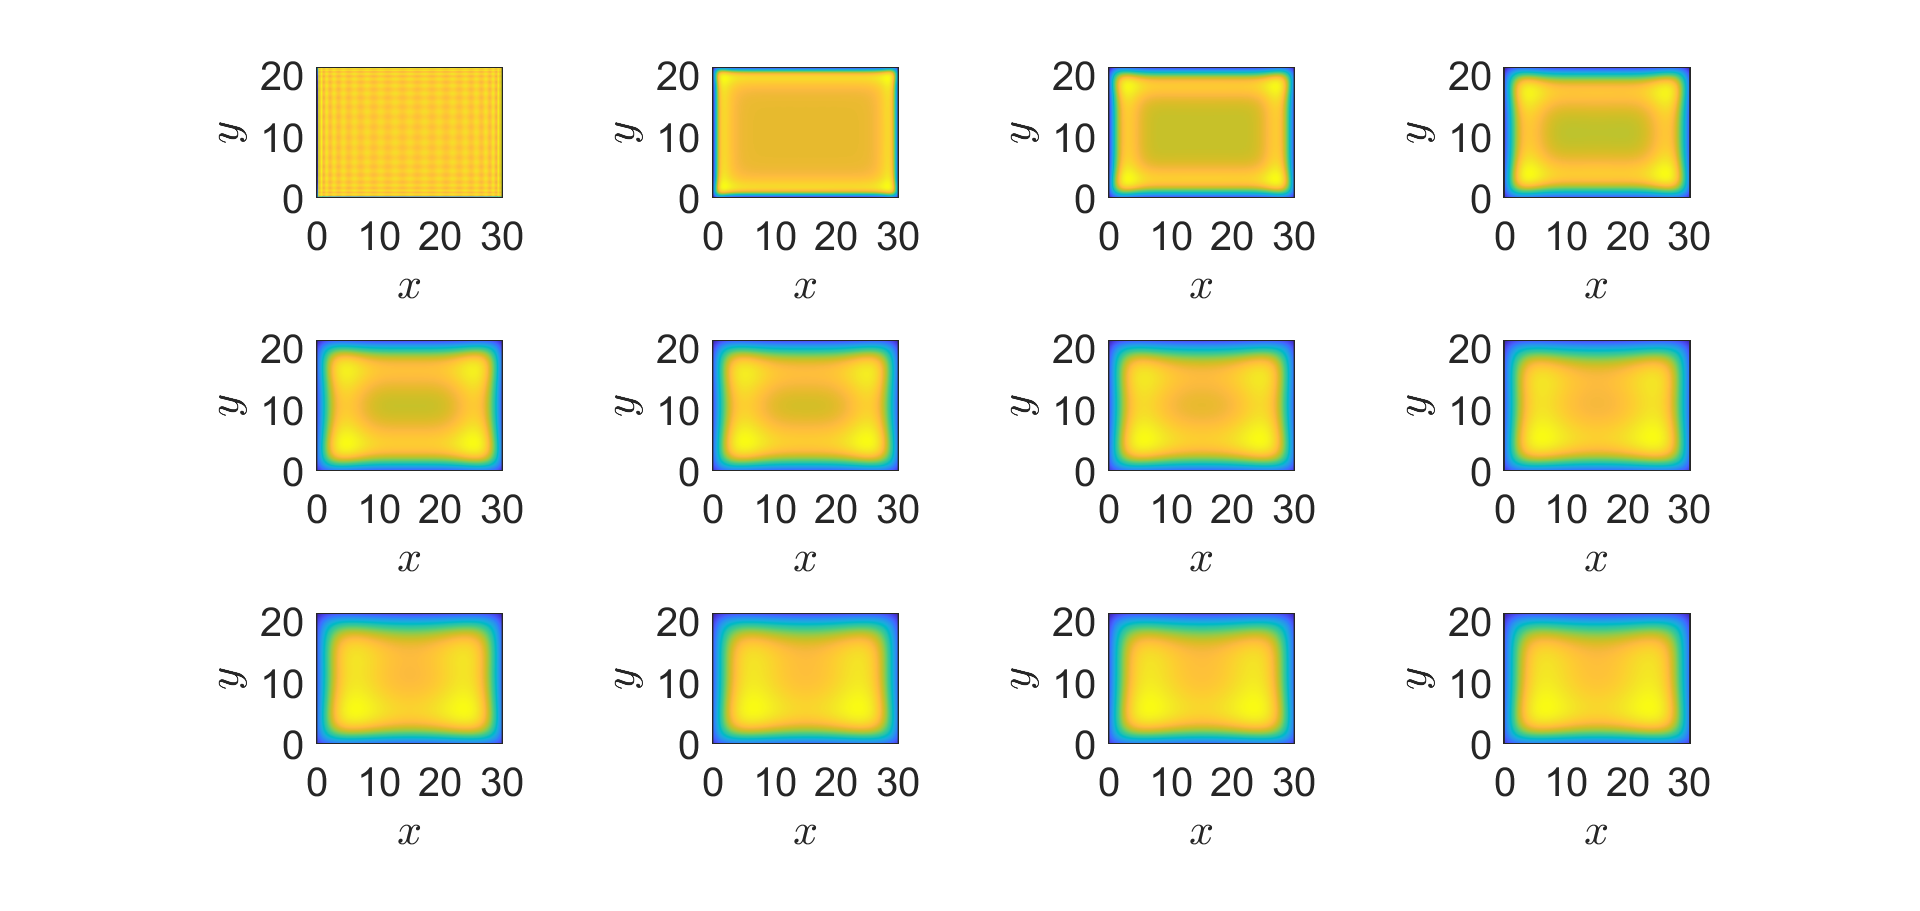
\includegraphics[scale=0.25]{F11.png}
	\caption{Ex1: Forward $\rho$ with $\w = \mathbf 0$} 
	\label{Fa1}
\end{figure}	
\begin{figure}[h]
	\centering
	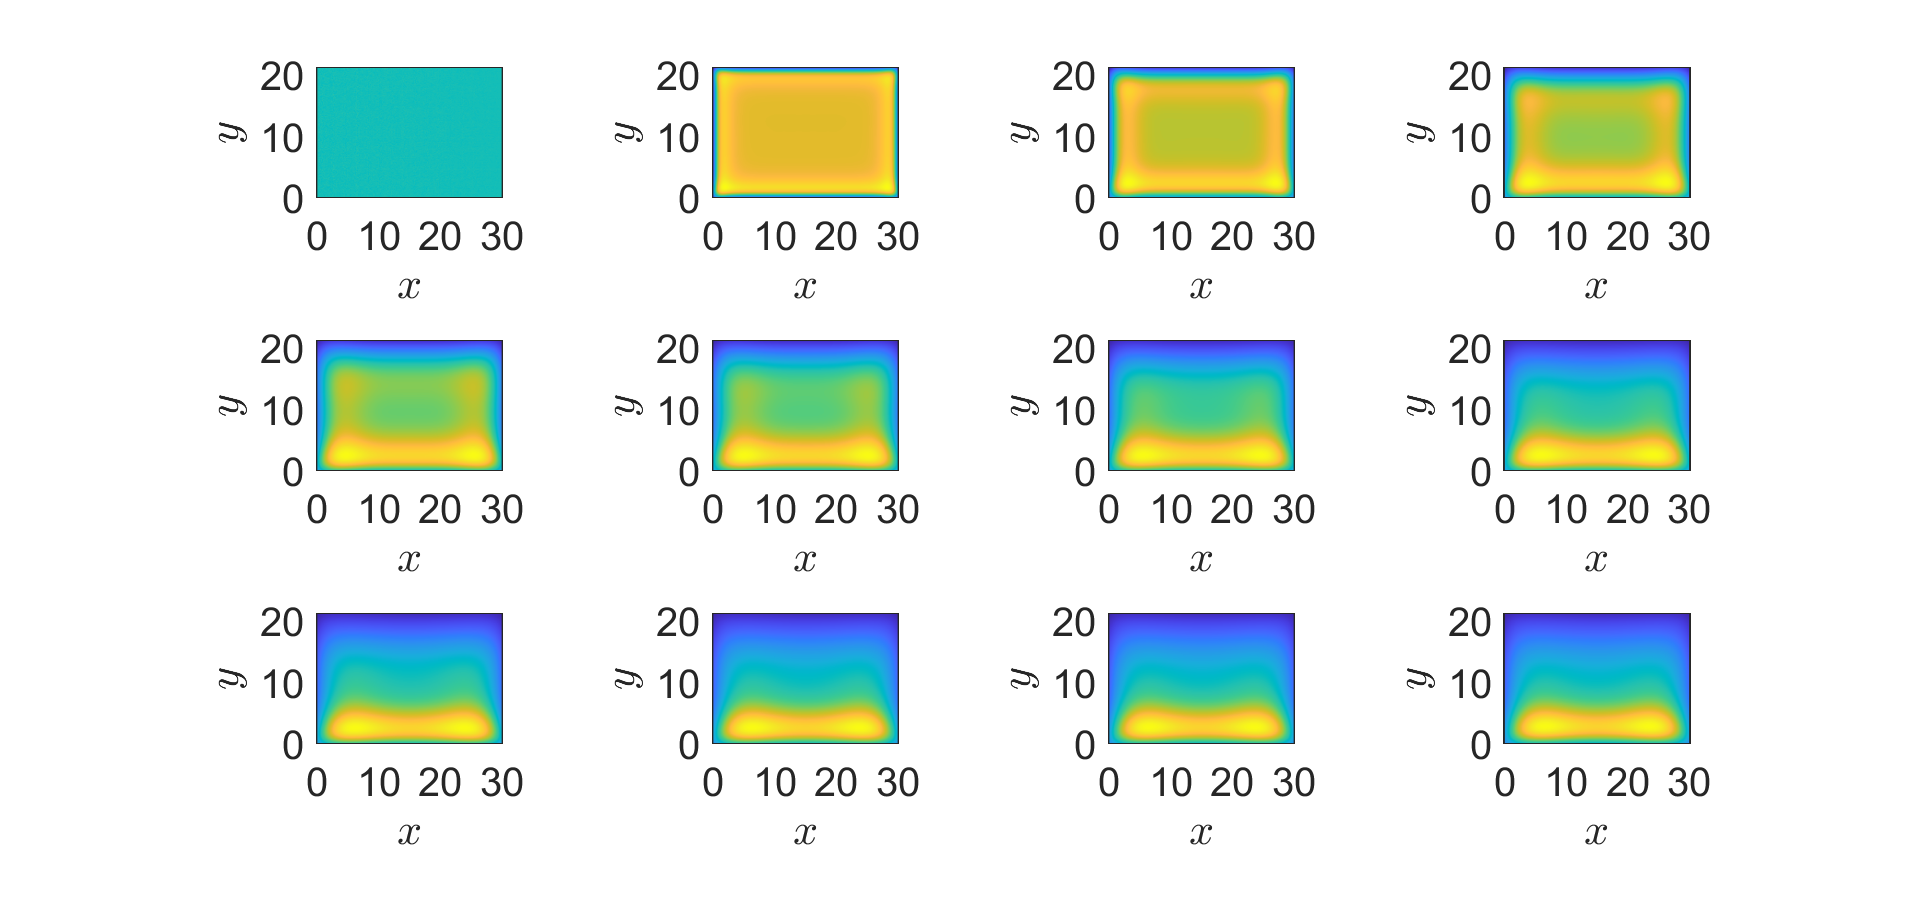
\includegraphics[scale=0.25]{F21.png}
	\caption{Ex1: Optimal $\rho$} 
	\label{Fa2}
\end{figure}
\begin{figure}[h]
	\centering
	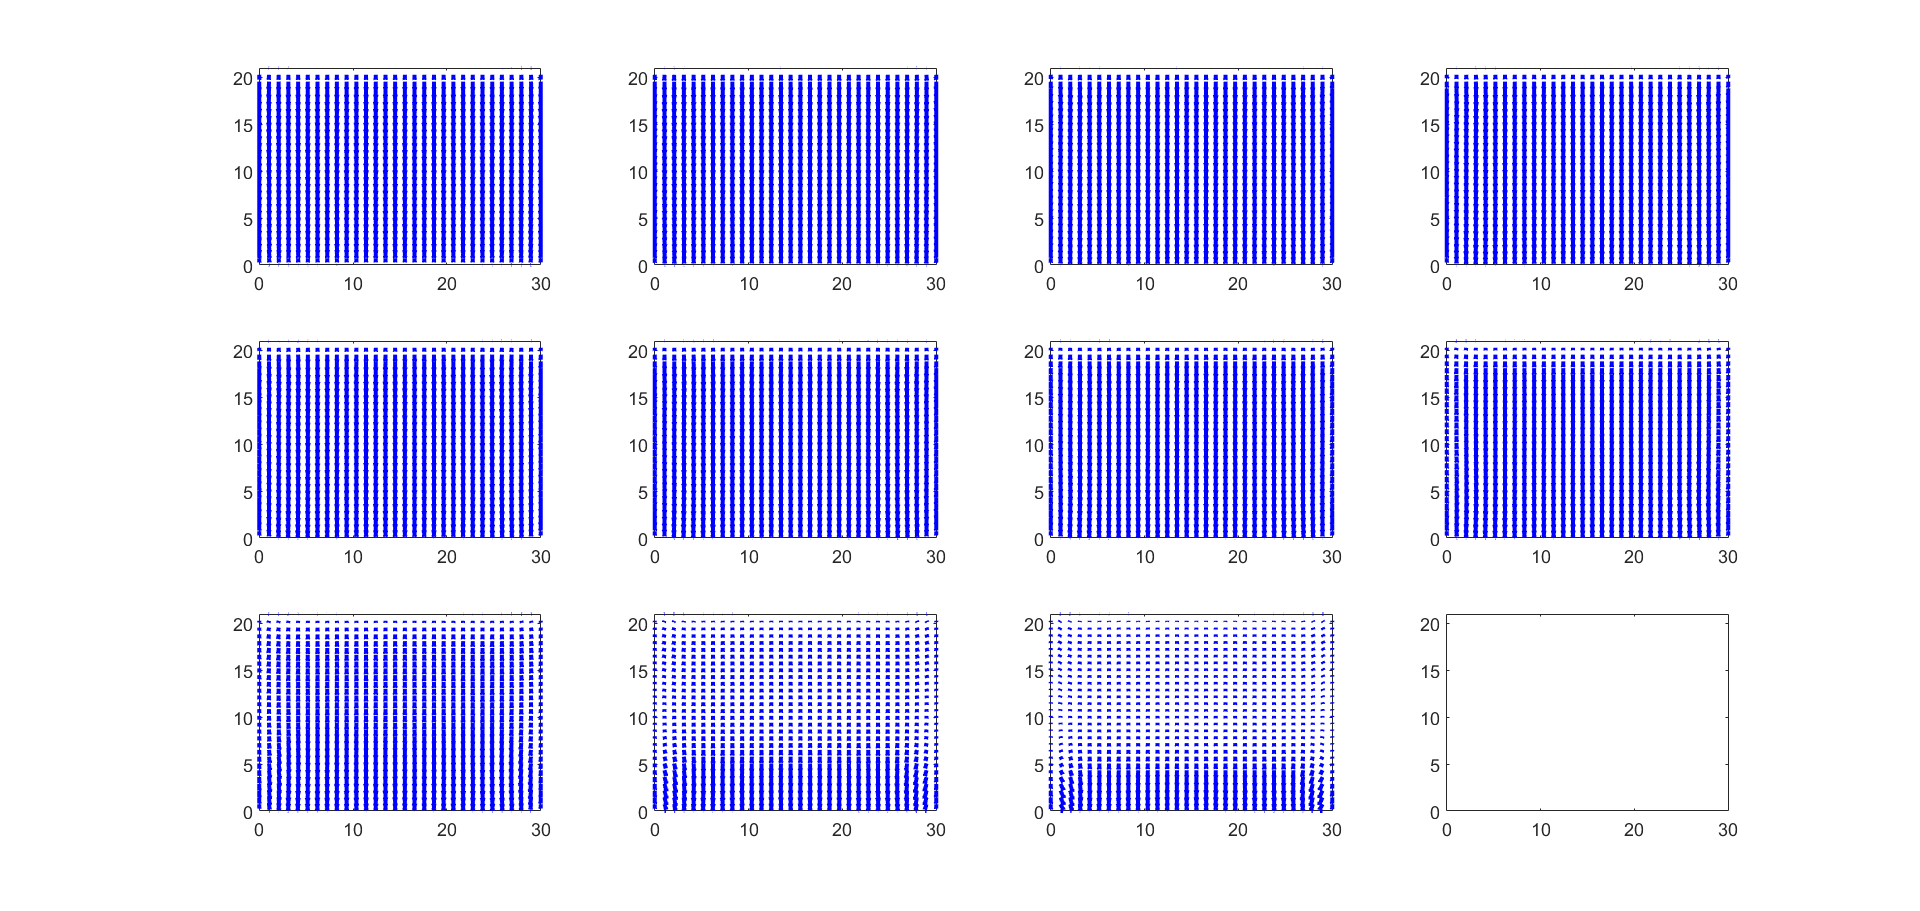
\includegraphics[scale=0.25]{F31.png}
	\caption{Ex1: Optimal Control} 
	\label{Fa3}
\end{figure}



\subsection{Optimization in a Box - Time-Independent Control}
We consider the identical problem but with the time-independent optimal control setup \eqref{eq:OCP2}, subject to the same constraint \eqref{eq:SedFWModel} with boundary conditions \eqref{eq:noFluxBCs}. This changes the gradient equation to the time independent version \eqref{eq:SedGradientEq2} and therefore we expect a control $\w$ which is averaged over the time horizon. Apart from this, we use the same setup as in the previous example, in terms of parameter choices. The baseline cost is $\mathcal J_{FW} = 0.4855$ and after optimizing this is lowered to $\mathcal J_{Opt} = 0.0733$. This is illustrated in Figures \ref{F7a} and \ref{F8a}. We observe that, as expected, $\mathcal J_{Opt}$ is larger than for the previous example where $\w$ was allowed to vary over time, since it is averaged over the time horizon.
	
\begin{figure}[h]
	\centering
	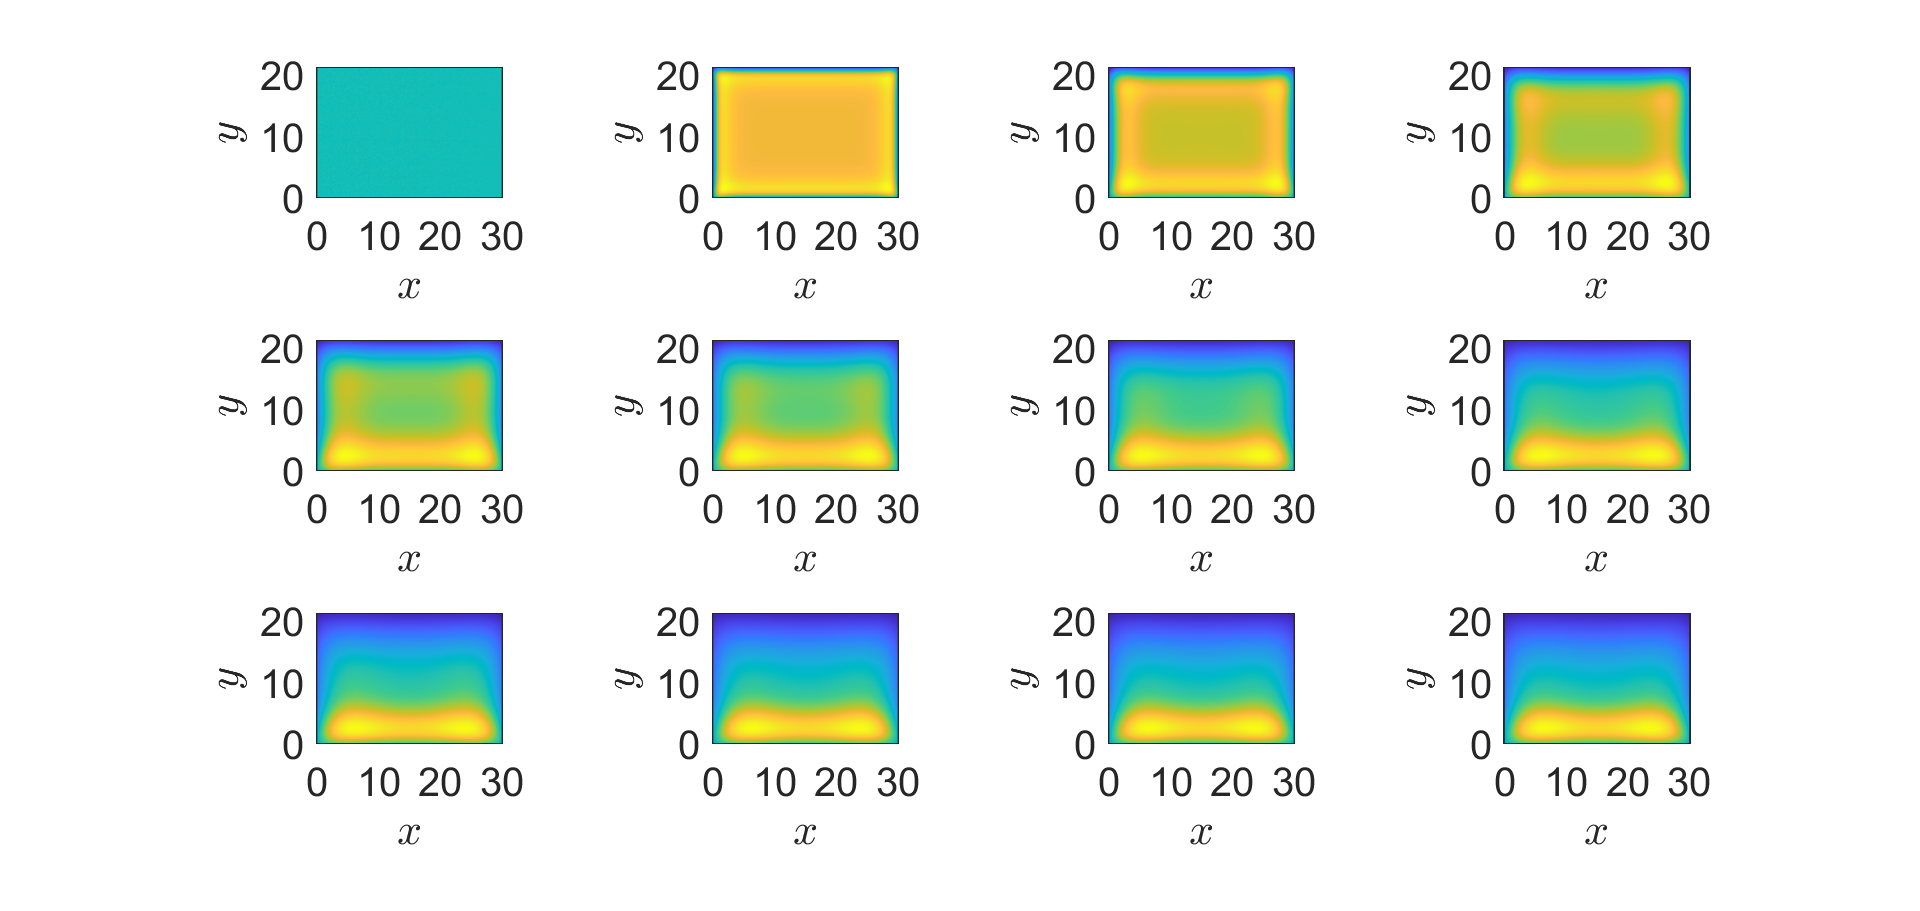
\includegraphics[scale=0.25]{C2.png}
	\caption{Ex2: Optimal $\rho$} 
	\label{F7a}
\end{figure}
\begin{figure}[h]
	\centering
	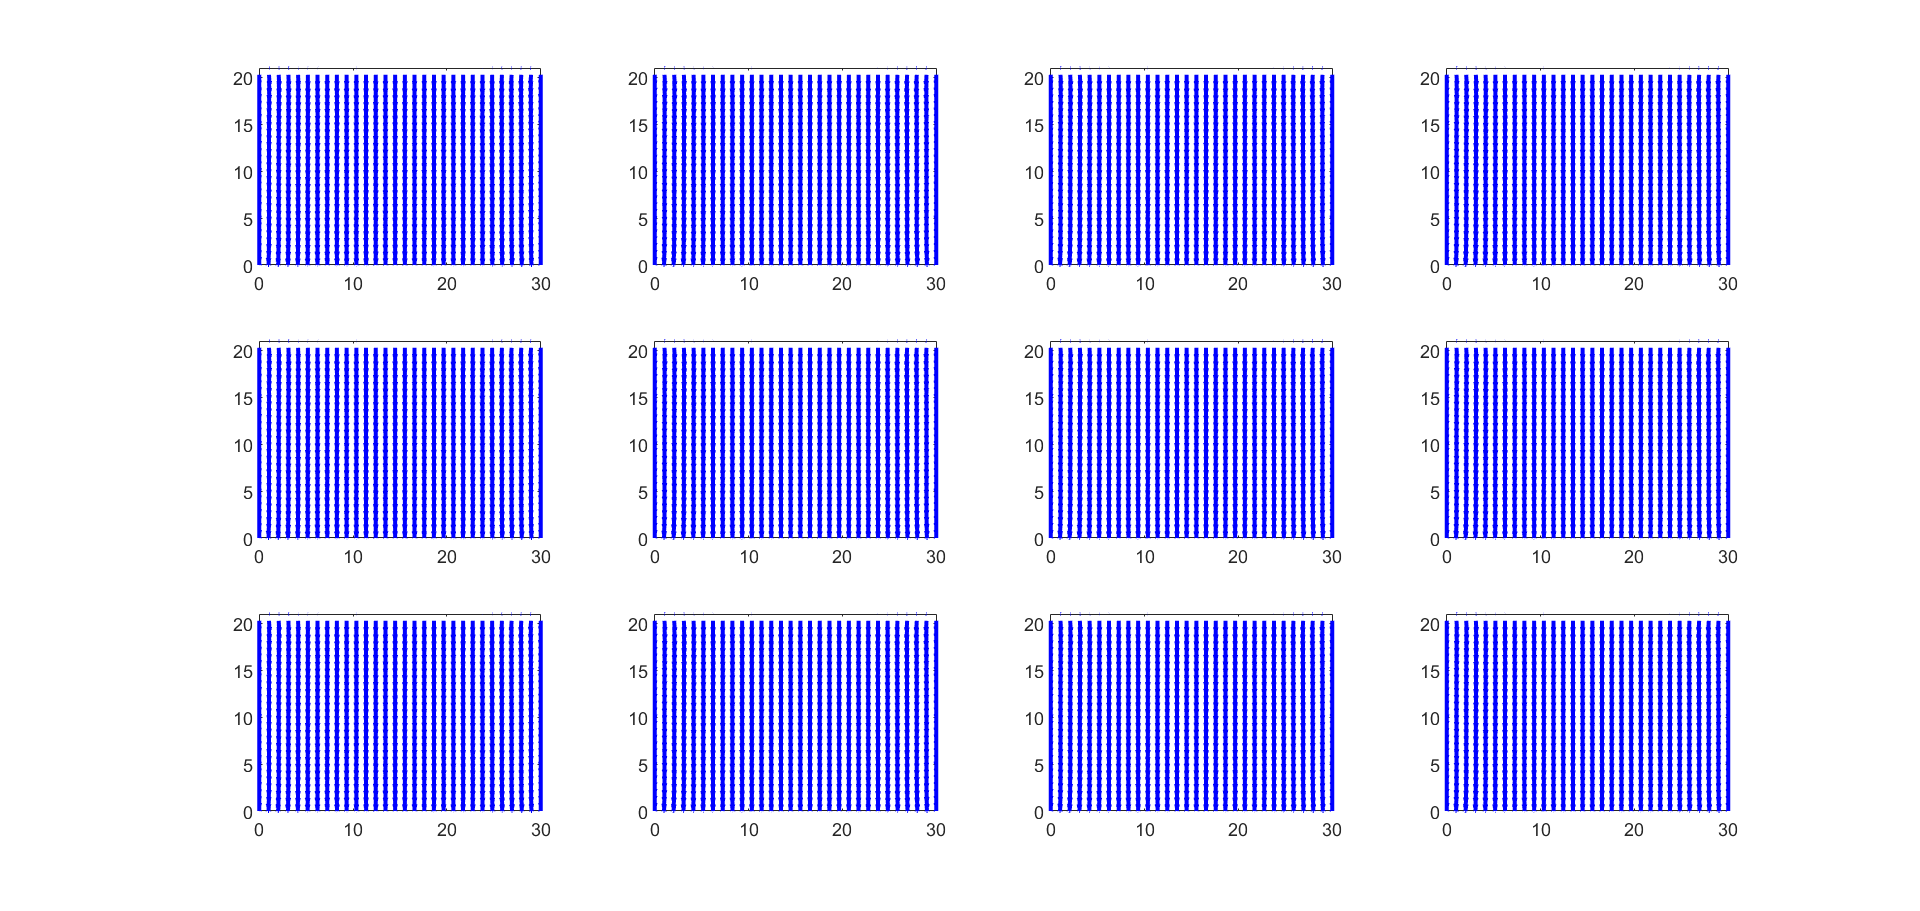
\includegraphics[scale=0.25]{C3.png}
	\caption{Ex2: Optimal Control} 
	\label{F8a}
\end{figure}

One obvious question to ask is whether the time independent flow control is similar to the $\nabla V_{ext}$ of the target, since this is what the control is trying to match. Figure \ref{F1a} shows the control and $\nabla V_{ext}$ of the target. We can see that one of these is positive, while the other one is negative. This is due to the opposite signs of $\w$ and $\nabla V_{ext}$ in the PDE. (++ needs to be fixed in plot ++) We observe that these two figures are very similar, however, the control is smaller than $\nabla V_{ext}$ at several points, showing that the overall energy applied to the system is smaller in the optimized problem than in the initial setup for the desired state $\hr$.

\begin{figure}[h]
	\centering
	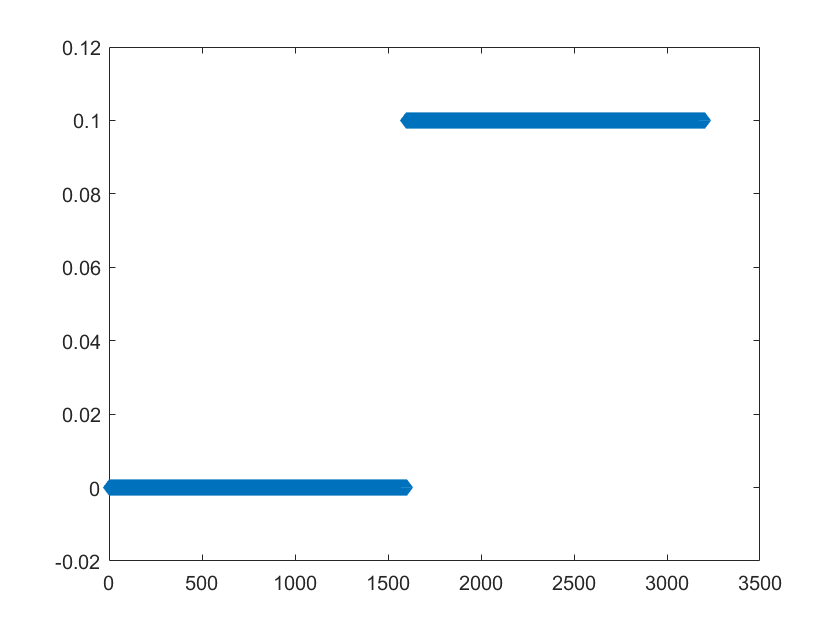
\includegraphics[scale=0.2]{V1.png}
	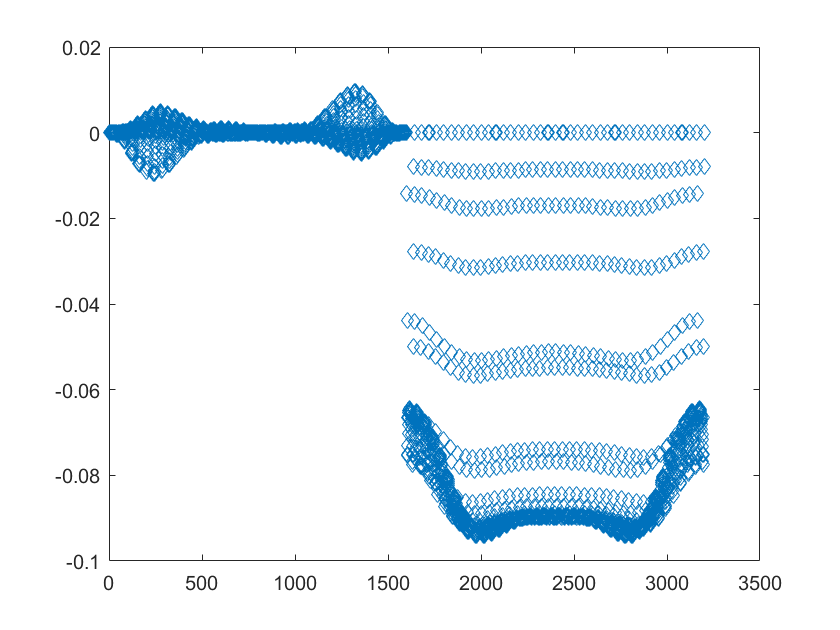
\includegraphics[scale=0.2]{W1.png}
	\caption{Ex2; $\nabla V_{ext}$ of the target $\hr$ and optimal control $\w$.} 
	\label{F1a}
\end{figure}

\subsection{Optimization on a Multishape}
We consider the time-dependent optimal control problem \eqref{eq:OCP1} subject to the constraint \eqref{eq:SedFWModel} with boundary conditions \eqref{eq:noFluxBCs}, but this time on a multishape, which is comprised of two quadrilaterals.
The setup remains the same as in the previous section, however, the time horizon only runs up to time $T = 30$. The resulting baseline cost is $\mathcal J_{FW} = 0.0713$ and the cost of the optimized problem is lowered to $\mathcal J_{Opt} = 0.0059$. The results are displayed in Figures \ref{FM0} and \ref{FM0a}.
\begin{figure}[h]
	\centering
	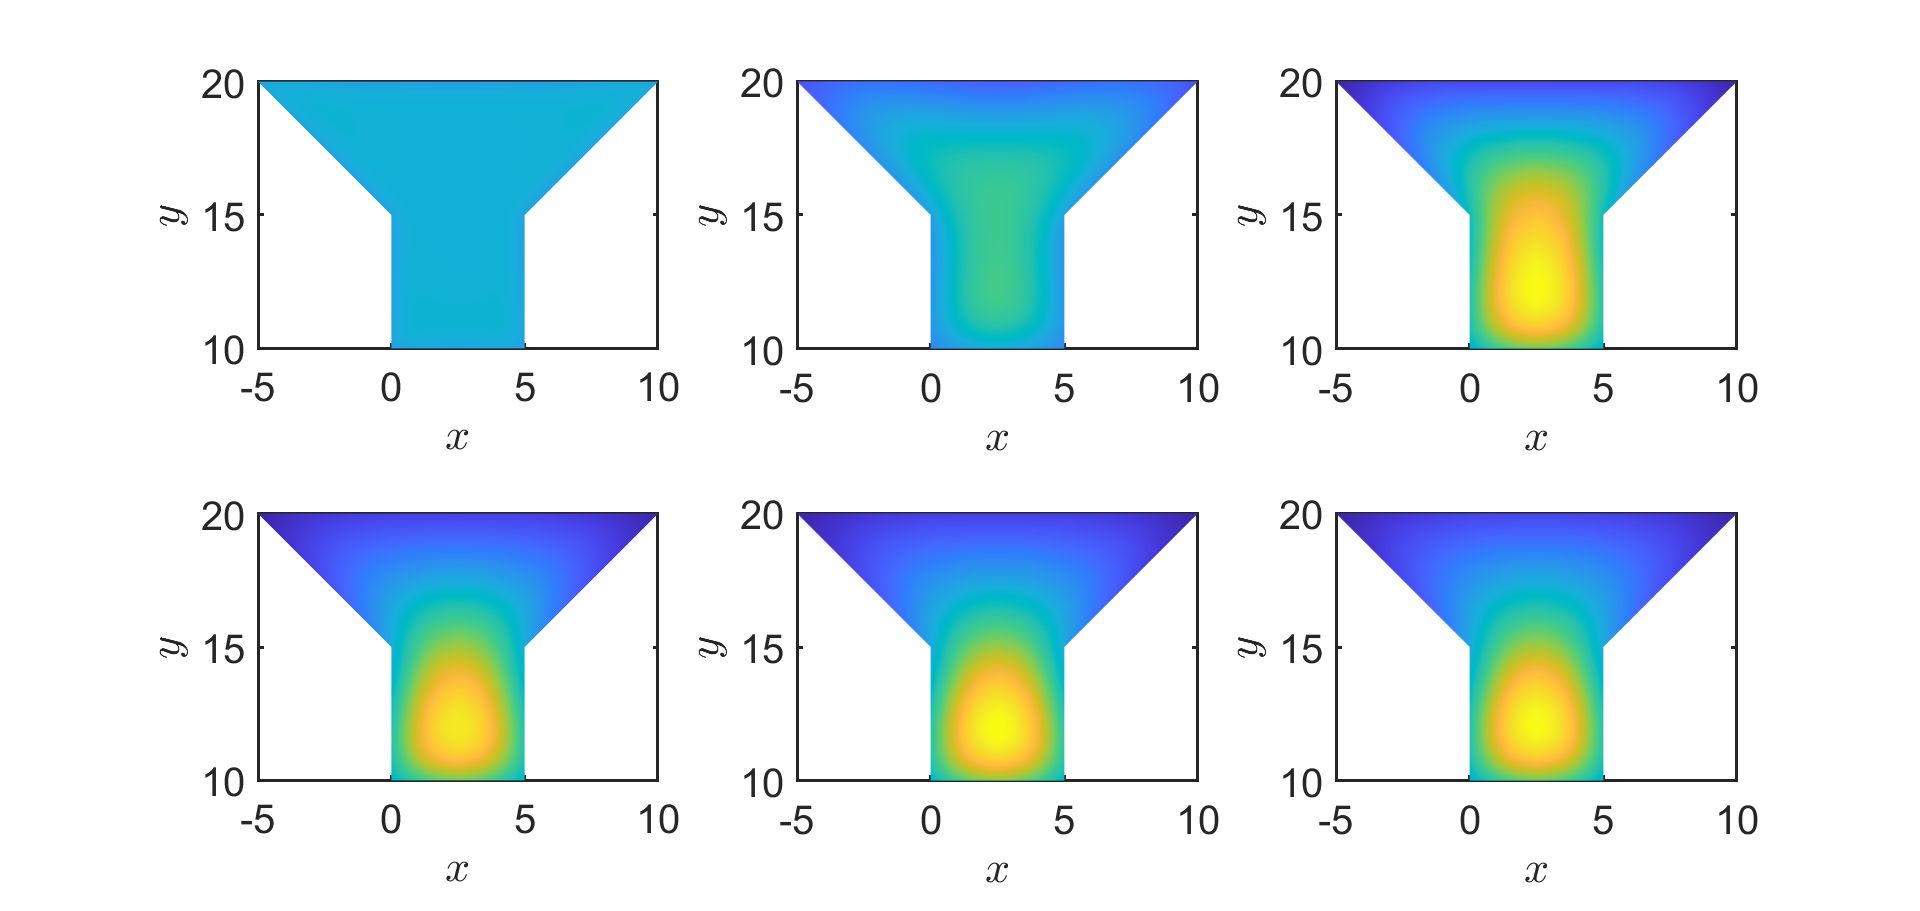
\includegraphics[scale=0.25]{MultiOpt1a.png}
	\caption{Ex31: Optimal $\rho$} 
	\label{FM0}
\end{figure}
\begin{figure}[h]
	\centering
	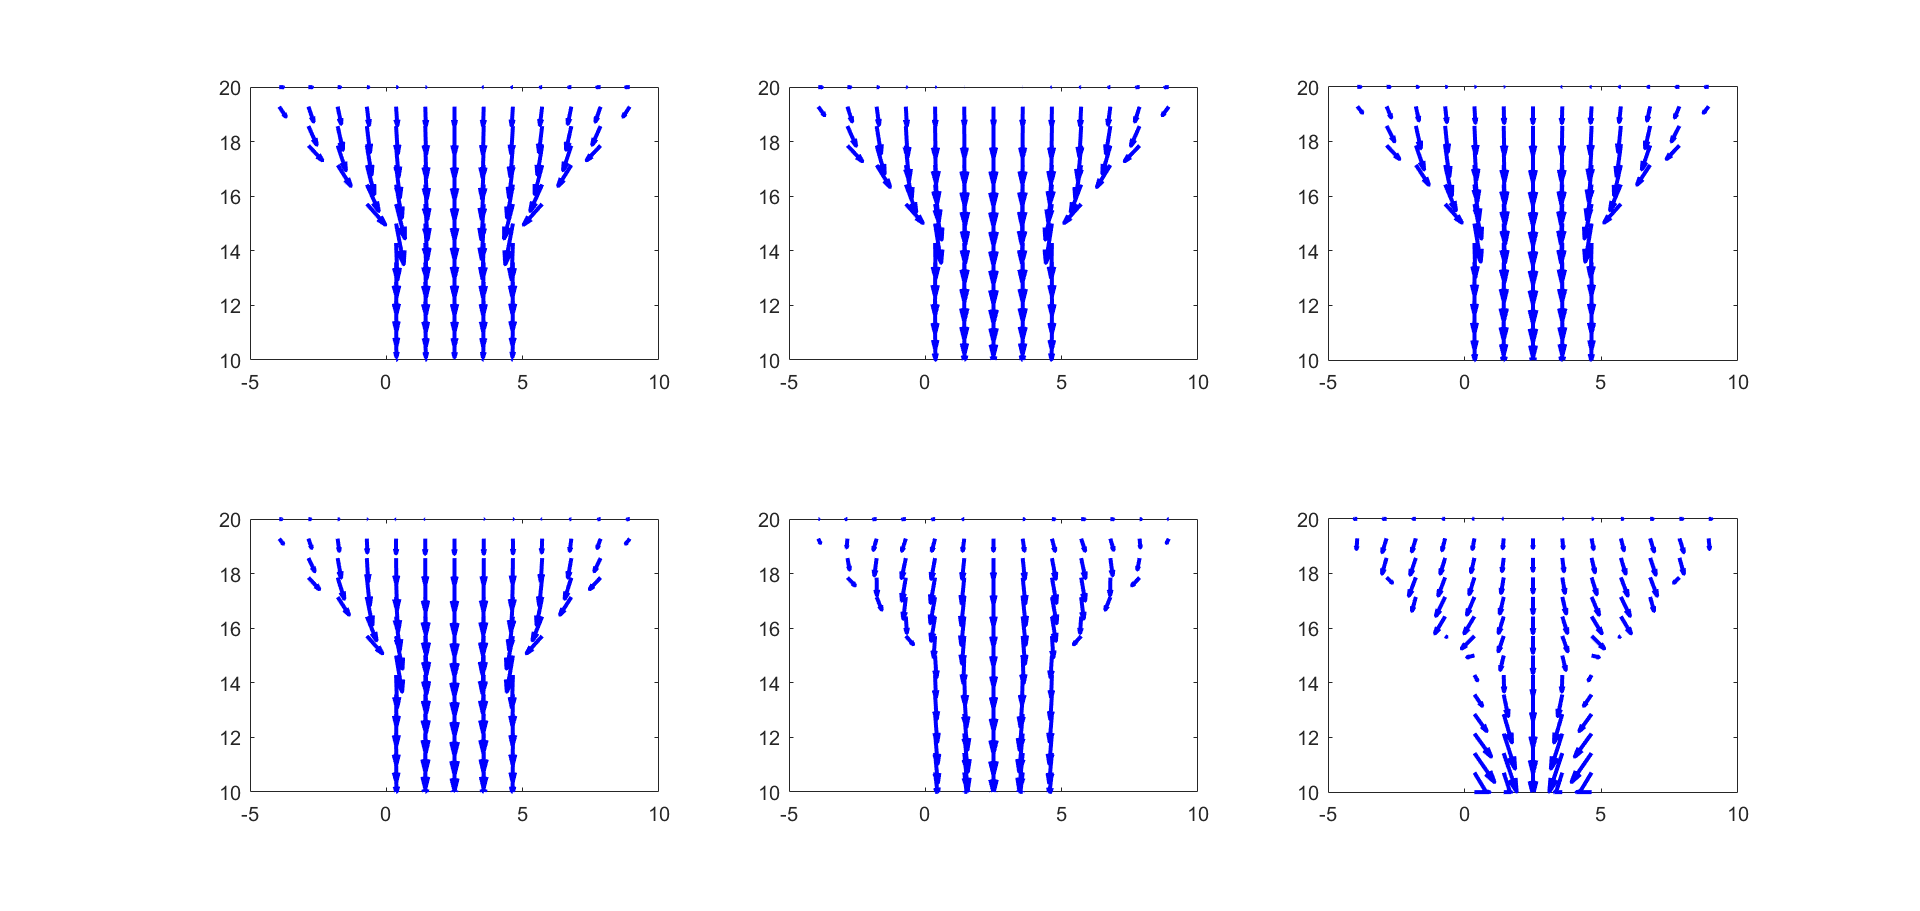
\includegraphics[scale=0.25]{MultiCont1a.png}
	\caption{Ex3: Optimal control} 
	\label{FM0a}
\end{figure}

For the fourth example, the setup remains the same as before, but now computed on a multishape which is comprised of four shapes, out of which three are quadrilaterals and one is a wedge. We compute an initial cost of $\mathcal J_{FW} = 0.0766$ and an optimized cost of $\mathcal J_{Opt} = 0.0116$. The results can be seen in Figures \ref{FM1a} and \ref{FM2a}.
\begin{figure}[h]
	\centering
	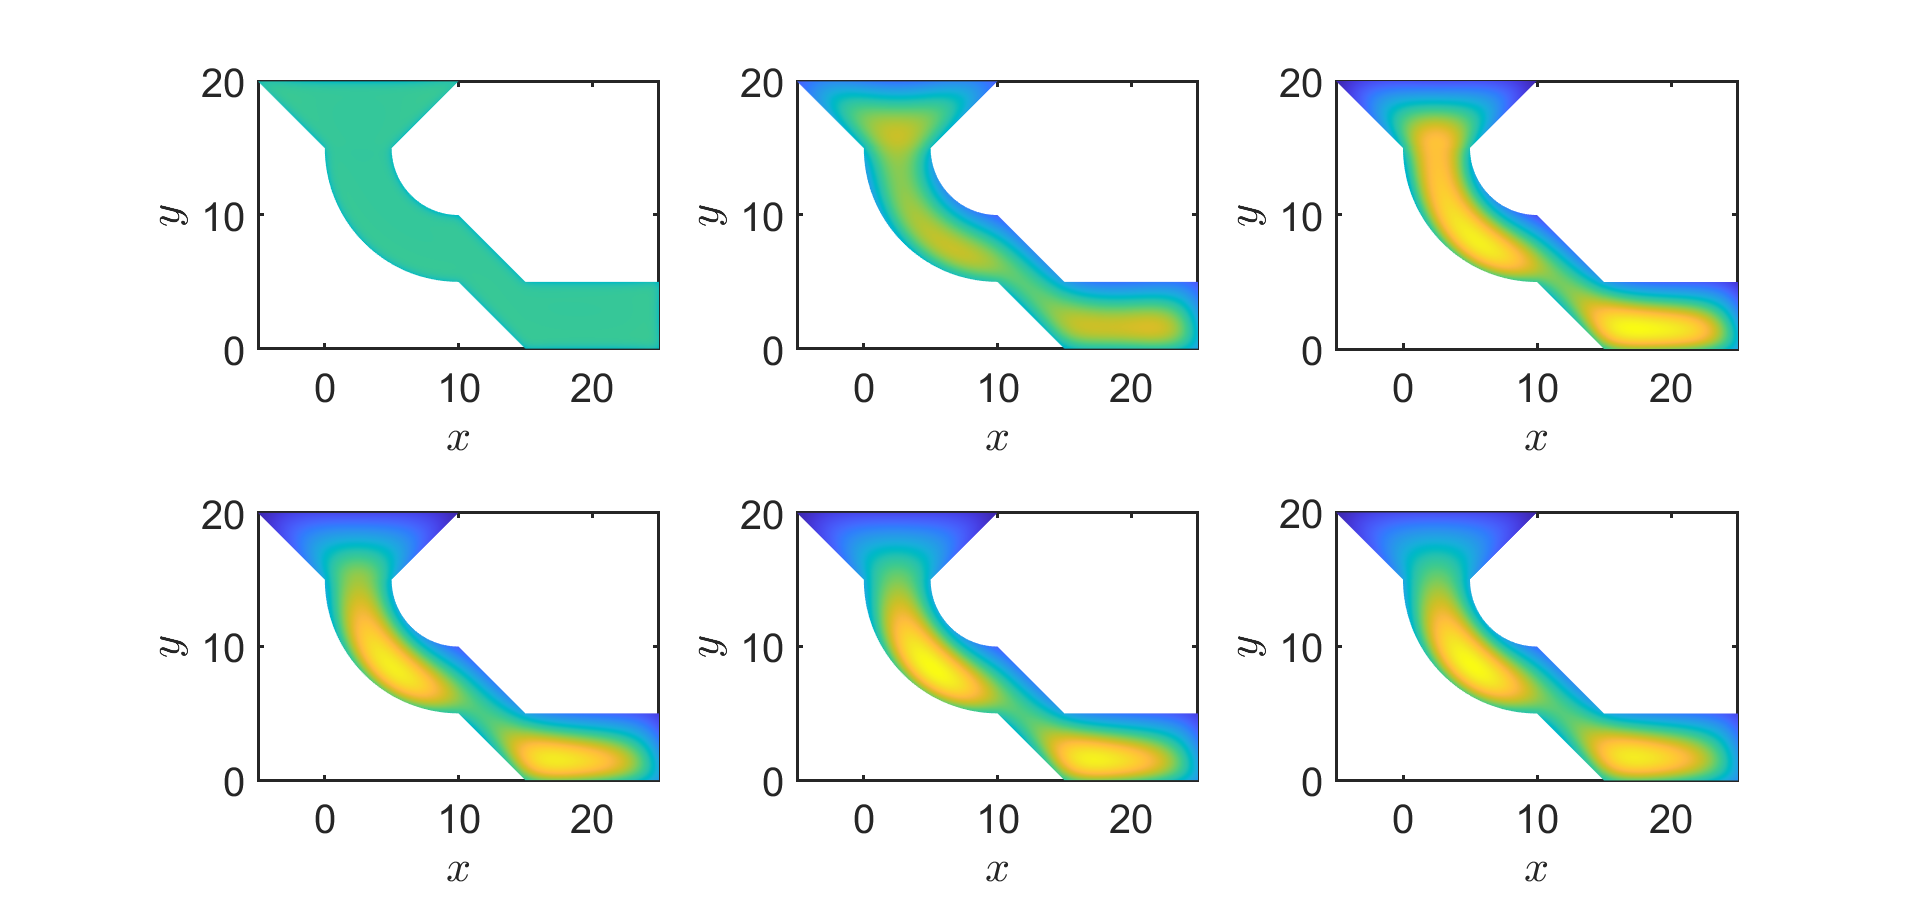
\includegraphics[scale=0.25]{MultiOpt2.png}
	\caption{Ex4: Optimal $\rho$} 
	\label{FM1a}
\end{figure}
\begin{figure}[h]
	\centering
	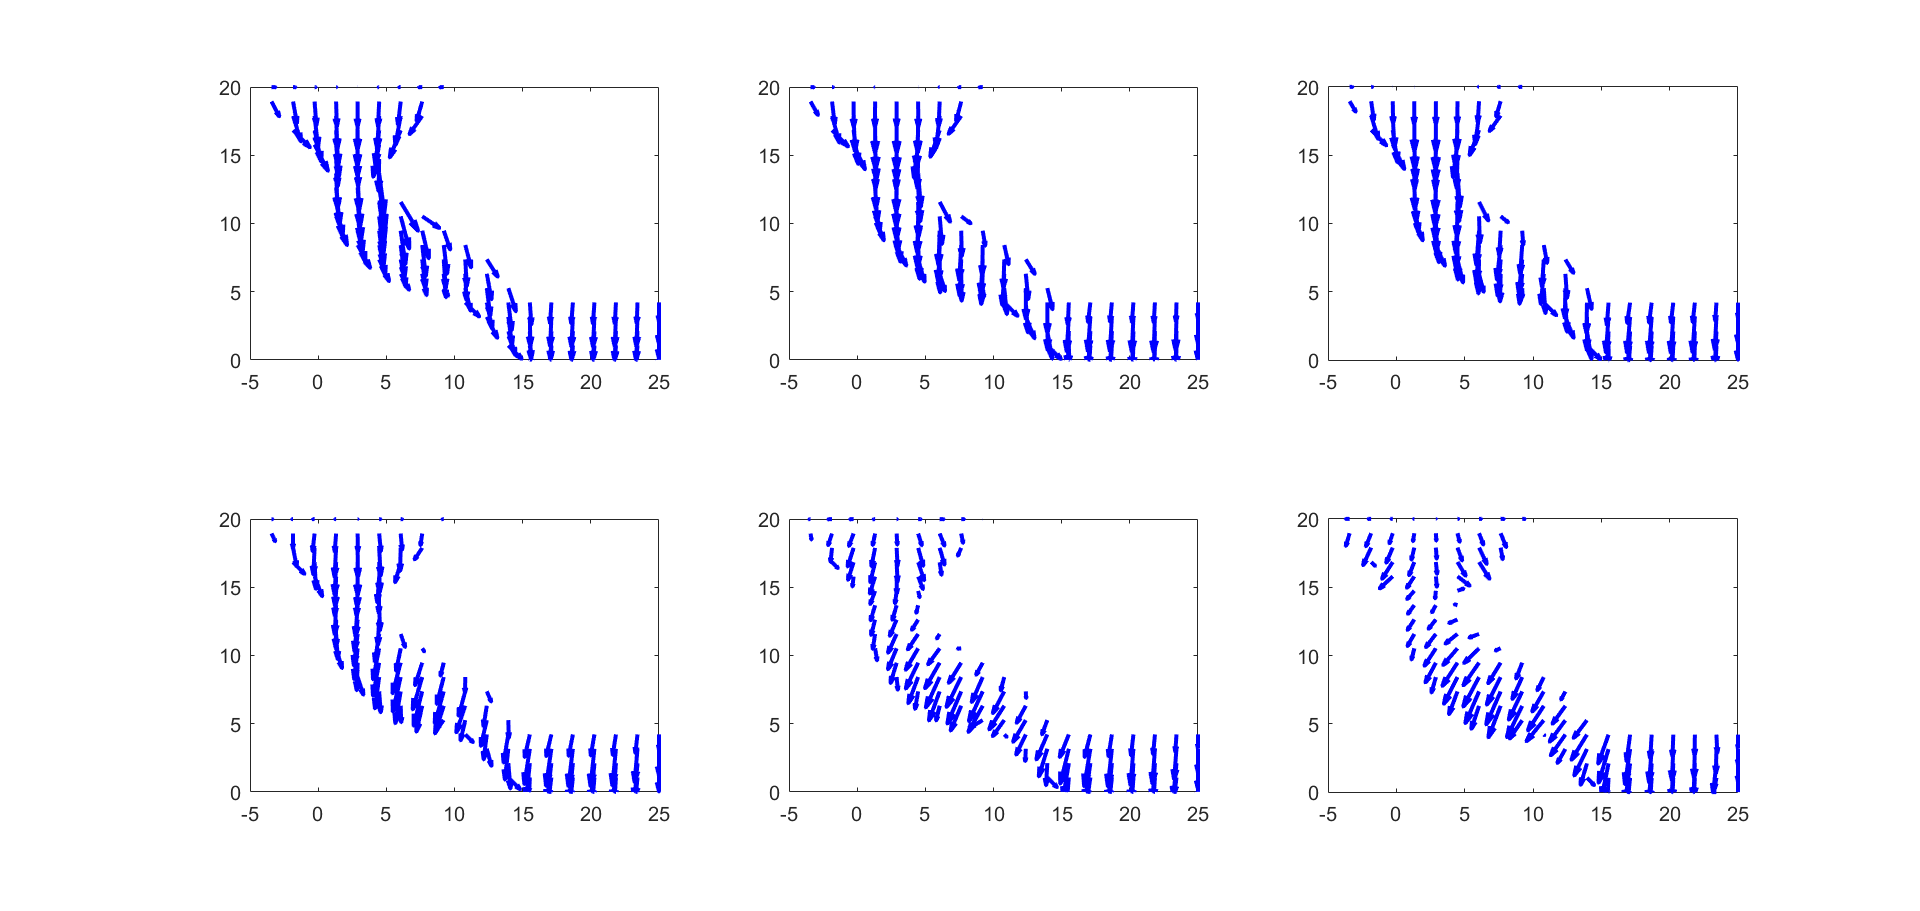
\includegraphics[scale=0.25]{MultiCont2.png}
	\caption{Ex4: Optimal control} 
	\label{FM2a}
\end{figure}

For a fifth example, we choose a multishape with an imposed background flow and gravity as a target. The optimal control problem has the same strength of gravity $c = 0.1$ imposed, but no flow. We expect the control to act similar to the flow profile imposed to produce $\hr$, see Figure \ref{FM3}. We choose $T = 10$ this time.
We get a baseline cost of $\mathcal J_{FW} = 0.0484$ and an optimized cost of $\mathcal J_{Opt} = 0.0258$. The results are illustrated in Figures \ref{FM3a} and \ref{FM3b}. Furthermore, we compare the strength of $\w$ of the target and the optimal control. The absolute $L_2$/ $L_\infty$ norms are compared, and we get $||\w_{\hr}|| = 68$ and $||\w_{Opt}|| = 50.8965$. This shows that the optimal control is indeed smaller than the control originally producing $\hr$, while still resulting in a $\rho$ close to the target state $\hr$.
\begin{figure}[h]
	\centering
	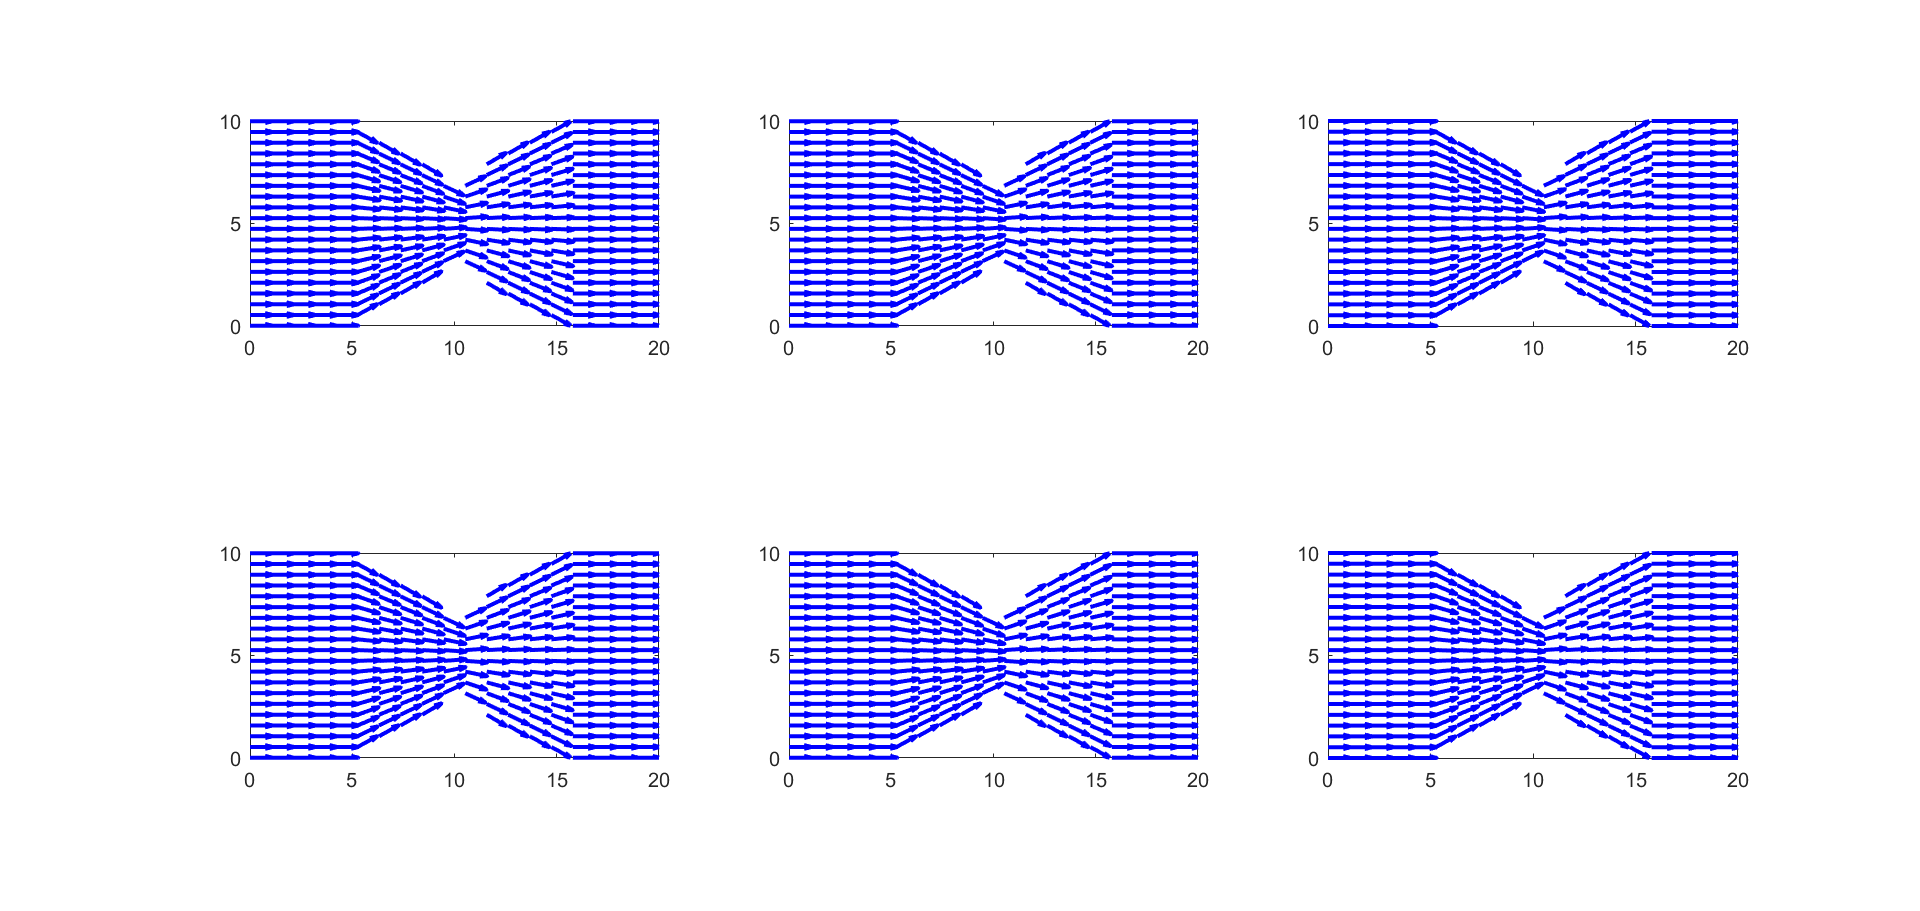
\includegraphics[scale=0.25]{MultiwFW.png}
	\caption{Multishape Example 3:Flow profile determining $\hr$} 
	\label{FM3}
\end{figure}
\begin{figure}[h]
	\centering
	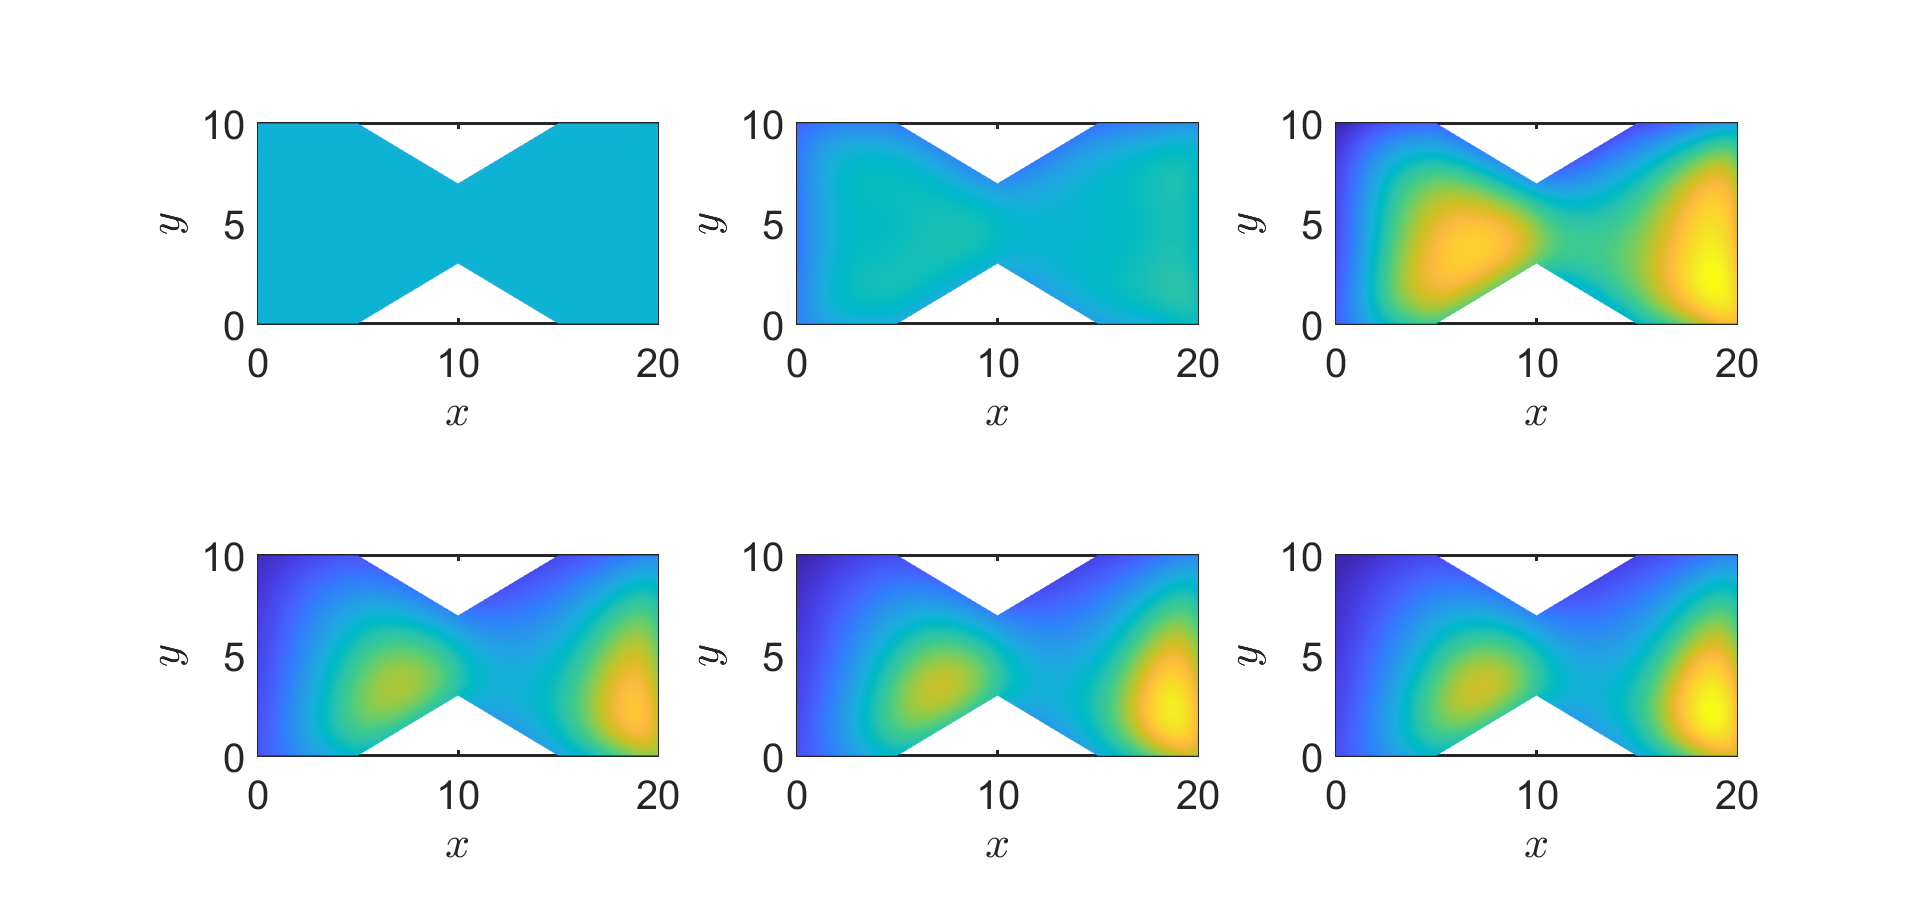
\includegraphics[scale=0.25]{MultiOpt3.png}
	\caption{Ex5: Optimal $\rho$} 
	\label{FM3a}
\end{figure}
\begin{figure}[h]
	\centering
	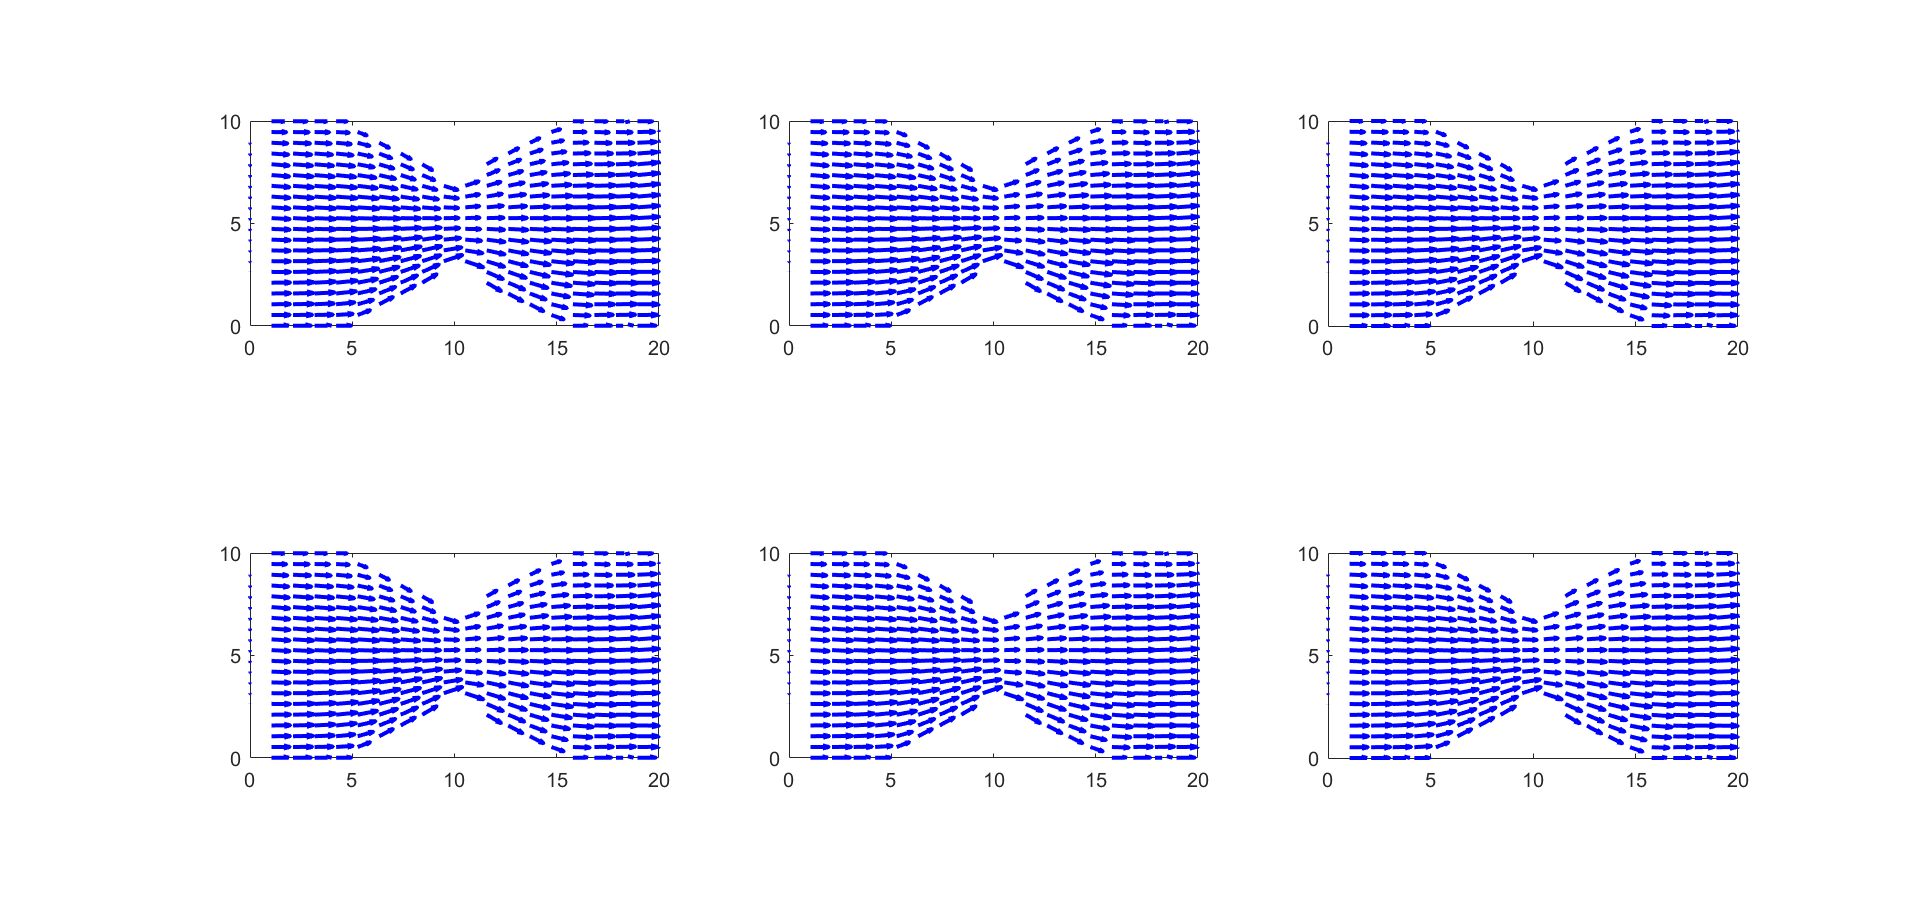
\includegraphics[scale=0.25]{MultiCont3.png}
	\caption{Ex5: Optimal control} 
	\label{FM3b}
\end{figure}

\subsection{Optimization on a Multishape - Time-Independent Control}
We consider the first multishape example from the previous section but with the time-independent optimal control setup \eqref{eq:OCP2}, subject to the same constraint \eqref{eq:SedFWModel} with boundary conditions \eqref{eq:noFluxBCs}. Here, since this is a more difficult problem, we choose $\lambda = 0.001$, which takes considerably more iterations than problems with larger $\lambda$.
We get a baseline cost of $\mathcal J_{FW} = 0.0713$ and an optimized cost of $\mathcal J_{Opt} = 0.0081$. The result can be seen in Figures \ref{FM1} and \ref{FM2}. If we compare with the time dependent case, as expected for the time independent control, the optimal cost is higher.



\begin{figure}[h]
	\centering
	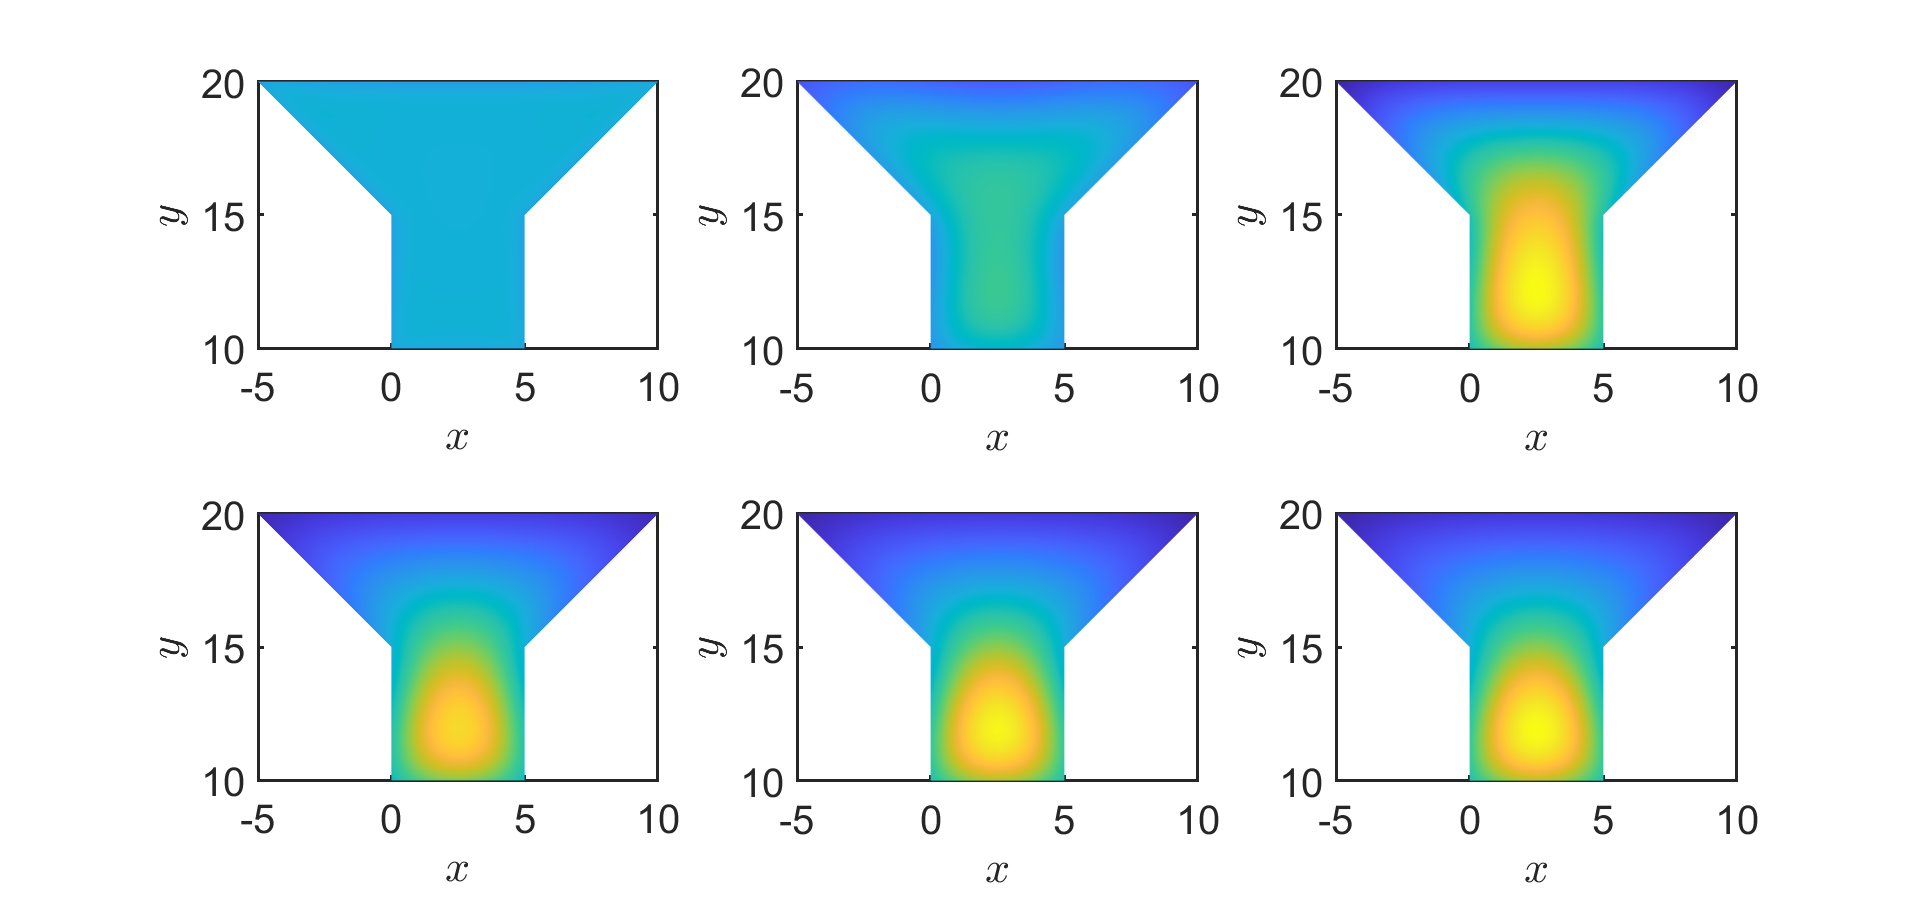
\includegraphics[scale=0.25]{MultiOpt1.png}
	\caption{Ex6: Optimal $\rho$} 
	\label{FM1}
\end{figure}
\begin{figure}[h]
	\centering
	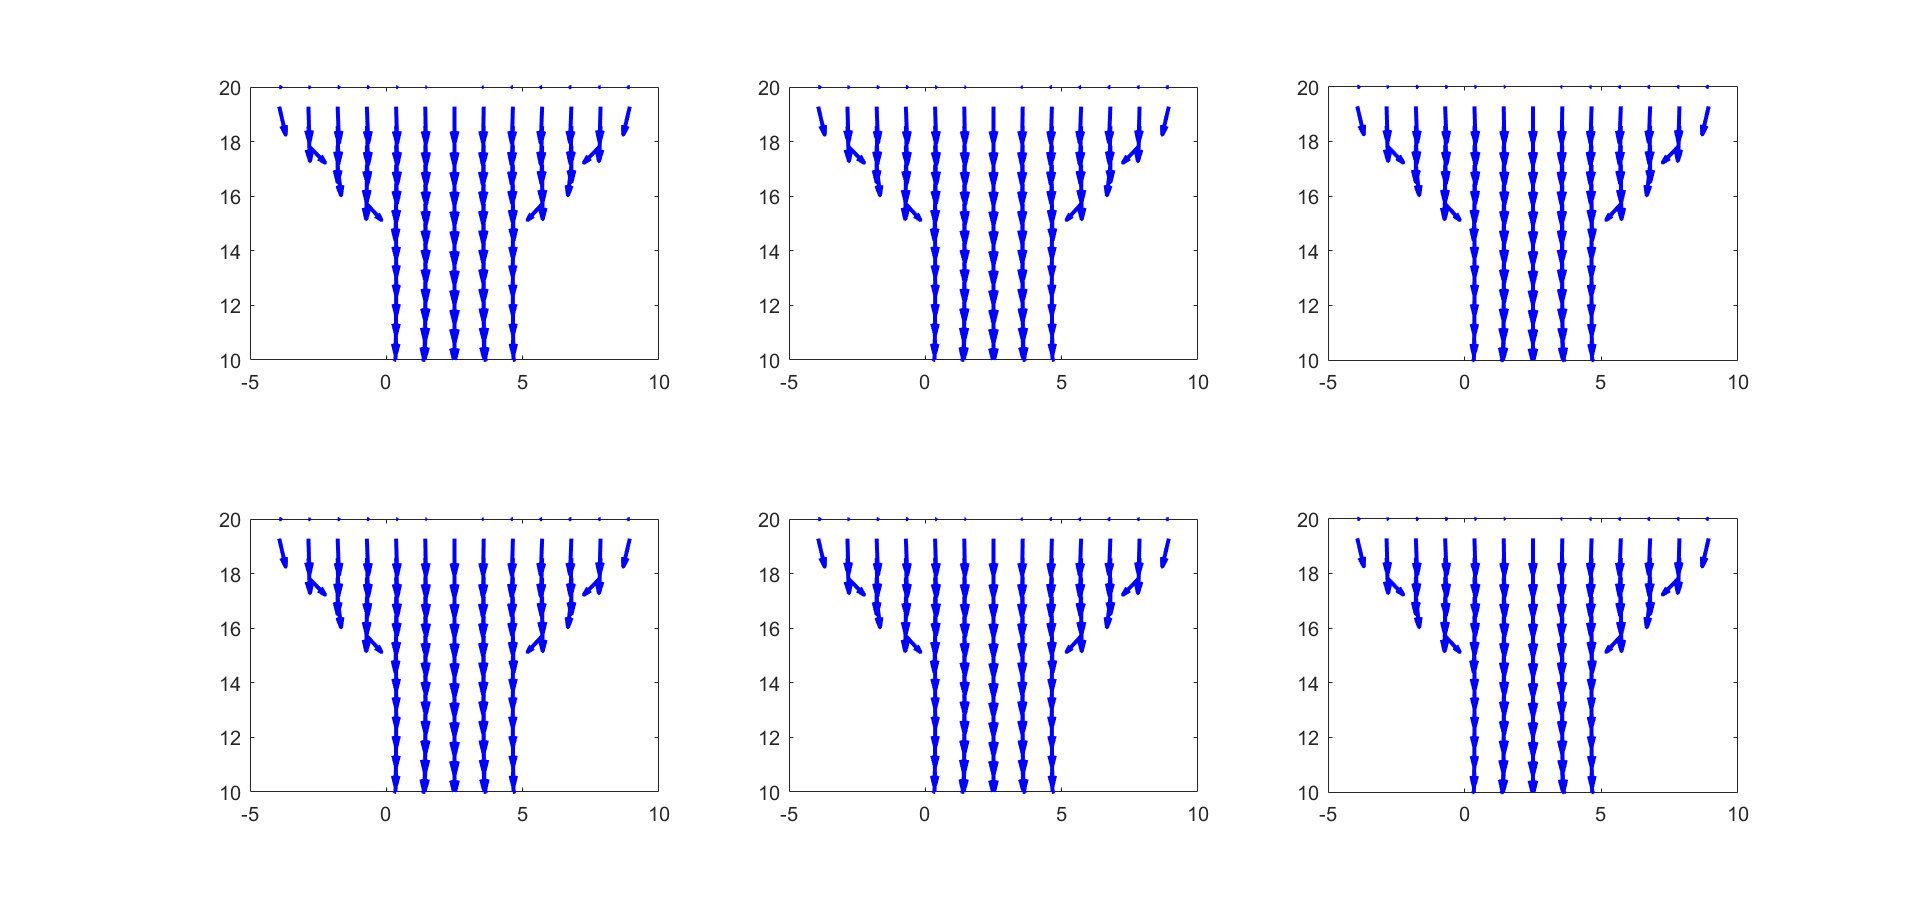
\includegraphics[scale=0.25]{MultiCont1.png}
	\caption{Ex6: Optimal control} 
	\label{FM2}
\end{figure}


\section{Concluding remarks}\label{sec:Conc}


\textbf{Acknowledgements.}~~
JCR is supported by The Maxwell Institute Graduate School in Analysis and
its Applications, a Centre for Doctoral Training funded by the UK Engineering and Physical Sciences Research Council (EPSRC grant EP/L016508/01), the Scottish Funding Council, Heriot-Watt University, and The University of Edinburgh.
%
BDG gratefully acknowledges support from the EPSRC grant EP/L025159/1.
%
JWP gratefully acknowledges support from the EPSRC Fellowship EP/M018857/2, the EPSRC grant EP/S027785/1, and a Fellowship from The Alan Turing Institute. 


\bibliographystyle{plain}
\bibliography{GeneralBib}
\end{document}